\begin{frame}[c]
    \frametitle{基于色散孔阵列衍射的微型光谱仪:概要}
    \begin{columns}
        \begin{column}{.6\textwidth}
            \begin{itemize}
                \item Yang, T.;  Xu, C.;  Ho, H.-p.;  Zhu, Y.-y.;  Hong, X.-h.;  Wang, Q.-j.;  Chen, Y.-c.;  Li, X.-a.;  Zhou, X.-h.;  Yi, M.-d.; Huang, W., Miniature spectrometer based on \textcolor{purple}{diffraction} in a \textcolor{red}{dispersive hole array}. Optics Letters 2015, 40 (13), 3217-3220.
                \item \textcolor{blue}{重要性:}\begin{itemize}
                          \item 不涉及运动部件、体积小、分辨率高、光谱范围宽、成本低、数据采集速度快、可靠性高;
                          \item 可以通过提高外设的计算能力来实现高分辨率、宽动态范围和实时测量能力。
                      \end{itemize}
                \item \textcolor{blue}{意义:}可以应用于生物分子识别和生物传感或通过光学吸收、荧光和发射线表征的航空航天遥测的化学分析。
                \item \textcolor{blue}{瓶颈:}\begin{itemize}
                          \item 无法集成到实验室芯片设备中;
                          \item 对于更大功率的光源需要更大的孔尺寸。
                      \end{itemize}
            \end{itemize}
        \end{column}
        \begin{column}{.4\textwidth}
            \begin{figure}[!htb] %H为当前位置,!htb为忽略美学标准,htbp为浮动图形
                \centering %图片居中
                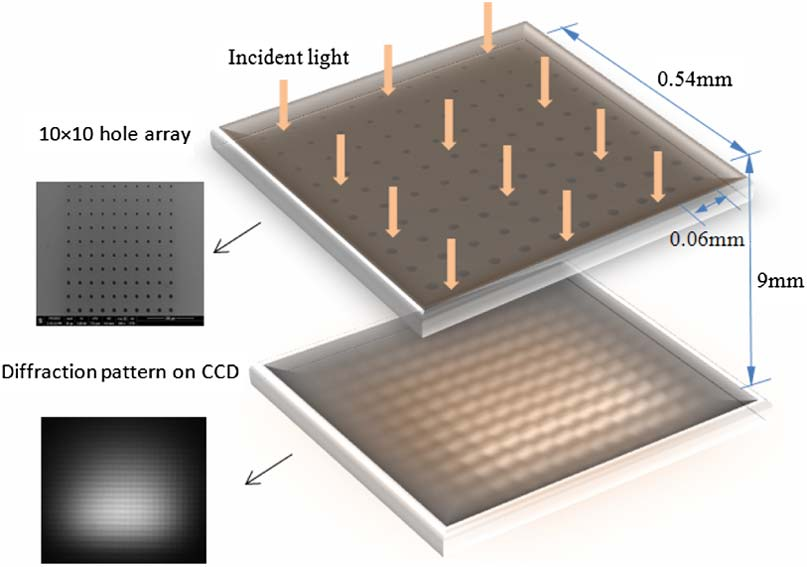
\includegraphics[width=1.\textwidth]{figures/Miniature spectrometer based on diffraction in a dispersive hole array_1.png} %插入图片,[]中设置图片大小,{}中是图片文件名
                \caption{器件结构示意图}
            \end{figure}
        \end{column}
    \end{columns}
\end{frame}

\begin{frame}[c]
    \frametitle{基于色散孔阵列衍射的微型光谱仪:性能}
    \begin{columns}
        \begin{column}{.5\textwidth}
            建议的使用方法:
            \begin{enumerate}
                \item 在较宽的光谱范围内初步粗略测量;
                \item 再在感兴趣的波长(峰值等)附近进行精细测量。
            \end{enumerate}
            \begin{itemize}
                \item 直接在过宽的光谱范围内测量的结果不够精确;
                \item 如果直接使用更多的散射孔进行测量,虽然精度可以达到要求,但是处理数据重构光谱的时间将会增长,不利于实时应用。
            \end{itemize}
        \end{column}
        \begin{column}{.5\textwidth}
            \begin{figure}[!htb] %H为当前位置,!htb为忽略美学标准,htbp为浮动图形
                \centering %图片居中
                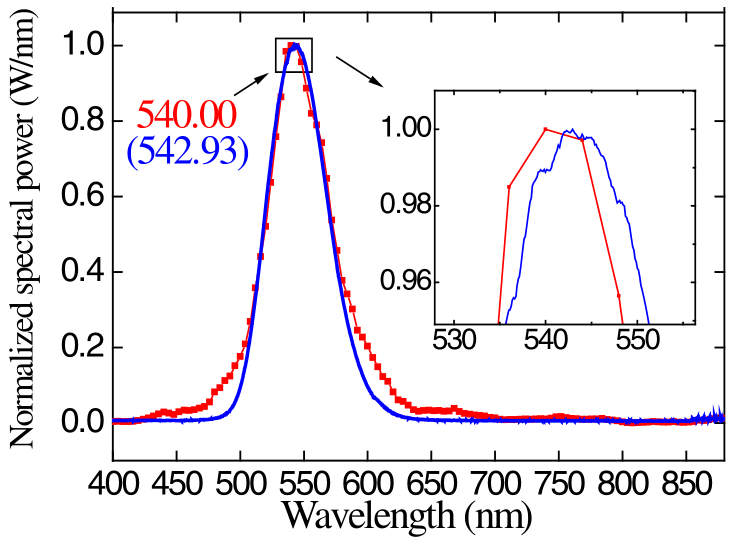
\includegraphics[width=1.\textwidth]{figures/Miniature spectrometer based on diffraction in a dispersive hole array_2.png} %插入图片,[]中设置图片大小,{}中是图片文件名
                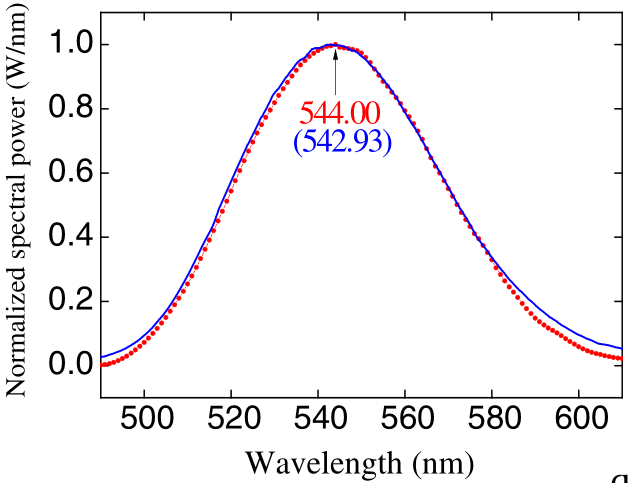
\includegraphics[width=1.\textwidth]{figures/Miniature spectrometer based on diffraction in a dispersive hole array_3.png} %插入图片,[]中设置图片大小,{}中是图片文件名
                \caption{测量顺序}
            \end{figure}
        \end{column}
    \end{columns}
\end{frame}

\begin{frame}[c]
    \frametitle{基于色散孔阵列衍射的微型光谱仪:原理}
    \begin{itemize}
        \item 假设有 $n$ 个探测器(接收器),则将入射光谱按波长分为 $n$ 段,有功率关系:\[P_0=\sum^{n}_{i=1}P(\lambda_i),\ i=1,2,\dots,n\]
        \item $C_{xi}$:第 $i$ 段光谱所包含的光在第 $x$ 块探测器上的功率;
        \item $P_x=\sum^{n}_{i=1}C_{xi}P(\lambda_i),\ x=1,2,\dots,n$
        \item \[\begin{bmatrix}
                      P_1 \\P_2\\ \vdots \\ P_n
                  \end{bmatrix}=\begin{pmatrix}
                      C_{11} & C_{12} & \cdots & C_{1n} \\
                      C_{21} & C_{22} & \cdots & C_{2n} \\
                      \vdots & \vdots & \ddots & \vdots \\
                      C_{n1} & C_{n2} & \cdots & C_{nn} \\
                  \end{pmatrix}\begin{bmatrix}
                      P(\lambda_1) \\P(\lambda_2)\\ \vdots \\ P(\lambda_n)
                  \end{bmatrix}\]
        \item 理论上就是求逆矩阵,数值上涉及到稳定性等问题。
    \end{itemize}
\end{frame}

\begin{frame}[c]
    \frametitle{基于色散孔阵列衍射的微型光谱仪:类比至光学薄膜}
    \begin{itemize}
        \item 假设有 $n$ 个(带光学薄膜的)探测器(接收器),则将入射光谱按波长分为 $n$ 段,有功率关系:\[P_0=\sum^{n}_{i=1}P(\lambda_i),\ i=1,2,\dots,n\]
        \item $T_{xi}\equiv T_{x}(\lambda_i)$:第 $x$ 块光学薄膜对第 $i$ 段光谱所包含的光的透射率,亦即第 $i$ 段光谱所包含的光在第 $x$ 块(带光学薄膜的)探测器上的功率与原功率之比;
        \item $P_x=\sum^{n}_{i=1}T_{xi}P(\lambda_i),\ x=1,2,\dots,n$
        \item \[\begin{bmatrix}
                      P_1 \\P_2\\ \vdots \\ P_n
                  \end{bmatrix}=\begin{pmatrix}
                      T_{11} & T_{12} & \cdots & T_{1n} \\
                      T_{21} & T_{22} & \cdots & T_{2n} \\
                      \vdots & \vdots & \ddots & \vdots \\
                      T_{n1} & T_{n2} & \cdots & T_{nn} \\
                  \end{pmatrix}\begin{bmatrix}
                      P(\lambda_1) \\P(\lambda_2)\\ \vdots \\ P(\lambda_n)
                  \end{bmatrix}\]
        \item 对比:\begin{itemize}
                  \item 与色散孔阵列的矩阵 $C_{xi}$ 相比,光学薄膜的矩阵 $T_{xi}$ 计算更加方便,前者需要对大量的衍射结果进行求和,而后者只需根据 Fresnel 公式即可逐步计算出透射率;
                  \item 光学薄膜的设计与色散孔阵列相比更加有规律可循,并且,光学薄膜在设计好之后就已经知道它的矩阵 $T_{xi}$,但是色散孔阵列的矩阵 $C_{xi}$ 则需要在制造出之后由实验确定(理论计算可能过于复杂);
                  \item 光学薄膜的所需要的器件更多,制造更繁琐。
              \end{itemize}
    \end{itemize}
\end{frame}